\section{球落下実験 実験結果}
\label{sec:expData}

\subsection{密度・濃度による影響に関して}
本研究において,落下させる球の密度,擬塑性流体の質量濃度を変化させた.それぞれの質量濃度における,球の落下速度をFig.\ref{fig:0.05-0.2}-\ref{fig:1.5}に示す.横軸は経過時間$s$,縦軸は落下速度$m/s$である.

\begin{figure}[H]
    \centering
    \includegraphics[width=1.0\textwidth]{5-Results/0.05-0.2.eps}
    \caption{Velocity of a falling sphere made by (a)nylon in 0.05 wt.\% PAA solution, (b)aluminum, (c)alumina, (d)stainless,(e)brass in 0.2 wt.\% PAA solution.}
    \label{fig:0.05-0.2}
\end{figure}

\begin{figure}[H]
    \centering
    \includegraphics[width=1.0\textwidth]{5-Results/0.5-0.7.eps}
    \caption{Velocity of a falling sphere made by (a)aluminum, (b)alumina, (c)stainless,(d)brass in 0.5 wt.\% PAA solution, (e)aluminum, (f)alumina, (g)stainless,(h)brass in 0.7 wt.\% PAA solution.}
    \label{fig:0.5-0.7}
\end{figure}

\begin{figure}[H]
    \centering
    \includegraphics[width=1.0\textwidth]{5-Results/1.0-1.3.eps}
    \caption{Velocity of a falling sphere made by (a)aluminum, (b)alumina, (c)stainless,(d)brass in 1.0 wt.\% PAA solution, (e)aluminum, (f)alumina, (g)stainless,(h)brass in 1.3 wt.\% PAA solution.}
    \label{fig:1.0-1.3}
\end{figure}

\newpage

\begin{figure}[H]
    \centering
    \includegraphics[width=0.9\textwidth]{5-Results/1.5.eps}
    \caption{Velocity of a falling sphere made by (a)alumina, (b)stainless,(c)brass in 1.5 wt.\% PAA solution.}
    \label{fig:1.5}
\end{figure}

\subsection{球径による影響に関して}

球径を変化させた際の実験結果をFig.\ref{fig:diameter-0.5}-\ref{fig:diameter-0.2-1.3}に示す.横軸は経過時間$s$,縦軸は落下速度$m/s$である.

\begin{figure}[H]
    \centering
    \includegraphics[width=0.9\textwidth]{X-Appendix/diameter-0.5/diameter.eps}
    \caption{Velocity of a falling sphere in 0.5wt.\% PAA of (a)5mm, (b)15mm, (c)20mm.}
    \label{fig:diameter-0.5}
\end{figure}

\begin{figure}[H]
    \centering
    \includegraphics[width=1\textwidth]{X-Appendix/diameter/diameter.eps}
    \caption{Velocity of a falling sphere in 1.0wt.\% PAA of (a)8mm, (b)10mm, (c)11mm, (d)12mm, (e)13mm, (f)14mm, (g)15mm, (h)20mm.}
    \label{fig:diameter}
\end{figure}

\begin{figure}[H]
    \centering
    \includegraphics[width=1\textwidth]{X-Appendix/diameter-0.2_1.3/diameter.eps}
    \caption{Velocity of a falling sphere in 0.2wt.\% PAA of (a)5mm, (b)8mm, 1.3wt.\% PAA of (c)8mm, (d)15mm, (e)20mm.}
    \label{fig:diameter-0.2-1.3}
\end{figure}
